\chapter*{Appendix}
\todo{Print glossary entries when finalizing document.}
% Uncomment for sorted glossary definitions
% \printglossaries


\includepdf[landscape, pagecommand={}\label{appendix:cncf-landscape}]{9_appendix/figures/cncf-landscape.pdf}


\section{Experiment Overview}
\begin{table}[!t]
    \centering

    \begin{tabularx}{\textwidth}{l X}
    
        \toprule
        \multicolumn{2}{c}{\textbf{EXP 1 - HTTP Maximum Throughput}}  \\
        \toprule
        
        \textbf{Goal}
        & To find the maximum throughput each of the meshed configurations can achieve. \\
        \midrule
        
        \textbf{Methodology}
        & The load generator will run in an unrestricted mode and generate as much load as possible without holding back and without any request timeouts. The maximum throughput is determined by looking at the actual number of requests per second in the configuration was able to achieve. \\
        \midrule
        
        \textbf{Workload} 
        & HTTP (\cref{sec:experiments:design:workloads:http}) \\
        \midrule

        \multirow{1}{*}{\textbf{Factors}} 
        & \Gls{sm} configuration (\cref{sec:experiments:design:meshes}) \\
        \midrule
        
        \textbf{Reasoning}
        & This experiment will serve as a baseline to determine the maximum throughput of all meshed configurations. The results will be used to determine sensible defaults for the experiments with a pre-defined constant throughput. \\

        \bottomrule

    \end{tabularx}
    \caption[Experiment Design: Experiment 1.]{Experiment Design: Experiment 1.}
    \label{tab:experiment:design:01}
\end{table}
\begin{table}[!t]
    \centering

    \begin{tabularx}{\textwidth}{l X}
    
        \toprule
        \multicolumn{2}{c}{\textbf{EXP 2 - HTTP Constant Throughput}}  \\
        \toprule
        
        \textbf{Goal}
        & To evaluate how \gls{sm} configurations behave under varying levels of load. \\
        \midrule
        
        \textbf{Methodology}
        & The load generator will generate load in a constant and uniform throughput setting. This means that the load generator will produce a set number of requests per second and will not deviate or try to catch up when requests are not processed in time.  \\
        \midrule
        
        \textbf{Workload} 
        & HTTP (\cref{sec:experiments:design:workloads:http}) \\
        \midrule

        \multirow{2}{*}{\textbf{Factors}} 
        & \Gls{sm} configuration (\cref{sec:experiments:design:meshes}) \\
        & Requests per second \\
        \midrule
        
        \textbf{Reasoning}
        & This experiment evaluates the \gls{sm} configurations under similar levels of load. This allows us to compare these configurations to one another when they undergo the same workloads.  \\

        \bottomrule

    \end{tabularx}
    \caption[Experiment Design: Experiment 2.]{Experiment Design: Experiment 2.}
    \label{tab:experiment:design:02}
\end{table}
\begin{table}[!t]
    \centering

    \begin{tabularx}{\textwidth}{l X}
    
        \toprule
        \multicolumn{2}{c}{\textbf{EXP 3 - HTTP Payload Response}}  \\
        \toprule
        
        \textbf{Goal}
        & To evaluate how \gls{sm} configurations behave with varying payload sizes. \\
        \midrule
        
        \textbf{Methodology}
        & The load generator will produce HTTP requests to the target service, which in turn will respond with pre-determined payload sizes.  \\
        \midrule
        
        \textbf{Workload} 
        & HTTP (\cref{sec:experiments:design:workloads:http}) \\
        \midrule

        \multirow{2}{*}{\textbf{Factors}} 
        & \Gls{sm} configuration (\cref{sec:experiments:design:meshes}) \\
        & Payload size \\
        \midrule
        
        \textbf{Reasoning}
        & This experiment introduces several pre-determined payload sizes to evaluate the effects of additional application data being transferred in meshed environments. This allows us to study the effects and potential additional overheads extra data transferes may cause. \\

        \bottomrule

    \end{tabularx}
    \caption[Experiment Design: Experiment 3.]{Experiment Design: Experiment 3.}
    \label{tab:experiment:design:03}
\end{table}
\begin{table}[!t]
    \centering

    \begin{tabularx}{\textwidth}{l X}
    
        \toprule
        \multicolumn{2}{c}{\textbf{EXP 4 - gRPC Maximum Throughput}}  \\
        \toprule
        
        \textbf{Goal}
        & To evaluate how meshed configurations behave with alternative communication protocols. \\
        \midrule
        
        \textbf{Methodology}
        & The load generator will generate gRPC traffic towards the gRPC service and do so in an unrestricted manner, meaning it will try to generate as much load as possible without holding back and without enforcing any timeouts. The maximum throughput is determined by looking at the actual number of requests per second in the configuration was able to achieve. \\
        \midrule
        
        \textbf{Workload} 
        & gRPC (\cref{sec:experiments:design:workloads:grpc}) \\
        \midrule

        \multirow{1}{*}{\textbf{Factors}} 
        & \Gls{sm} configuration (\cref{sec:experiments:design:meshes}) \\
        \midrule
        
        \textbf{Reasoning}
        & This experiment allows us to evaluate the effects of alternative application level protocols. During the system survey we uncovered that \gls{sm} systems inspect and use this data to for both observability and routing functionalities. This experiment allows us to uncover the effects of alternative, but common, application level protocols widely used within the industry. \\

        \bottomrule

    \end{tabularx}
    \caption[Experiment Design: Experiment 4.]{Experiment Design: Experiment 4.}
    \label{tab:experiment:design:04}
\end{table}

\section{Experiment 1 Results}

\begin{figure}[h]
    \centering
    
    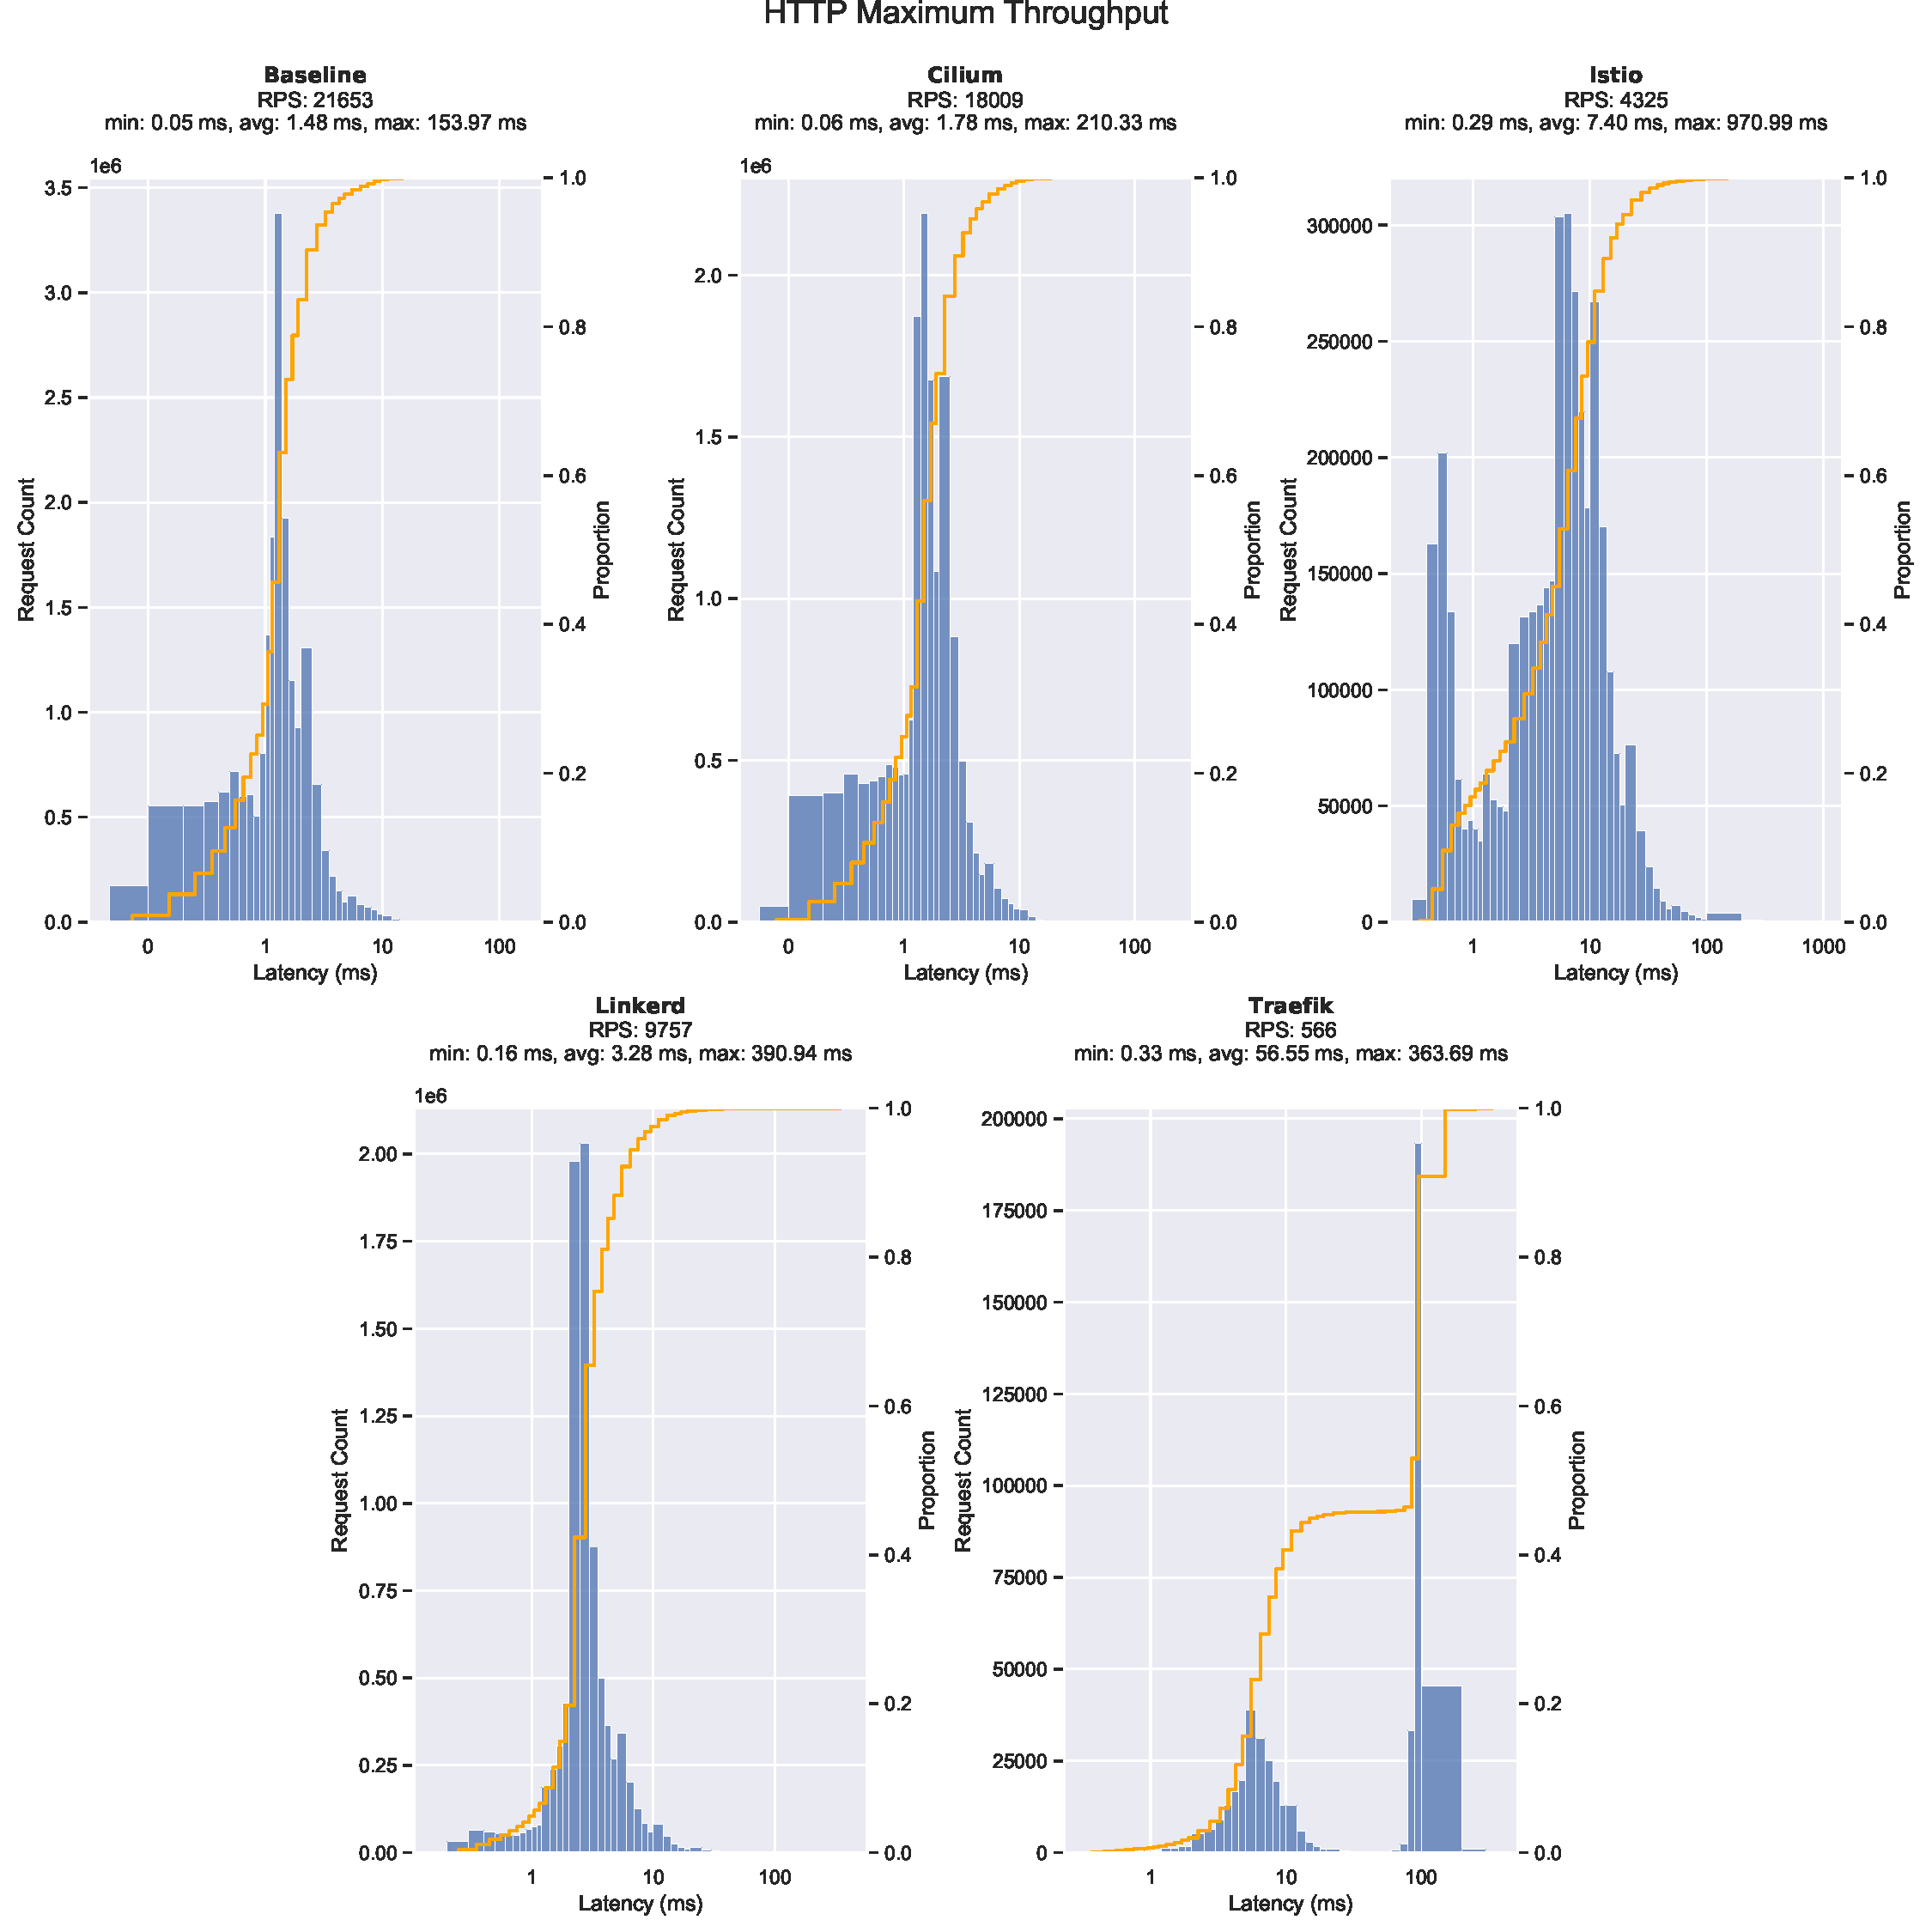
\includegraphics[width=\linewidth]{5_experimental_evaluation/figures/exp_01-latency-results.pdf}

    \caption{\ref{exp:design:1} - Histogram - Latency per Service Mesh.}
    
    \label{fig:appendix:exp:result:01:latency:histogram}
\end{figure}

\begin{figure}[h]
    \centering
    
    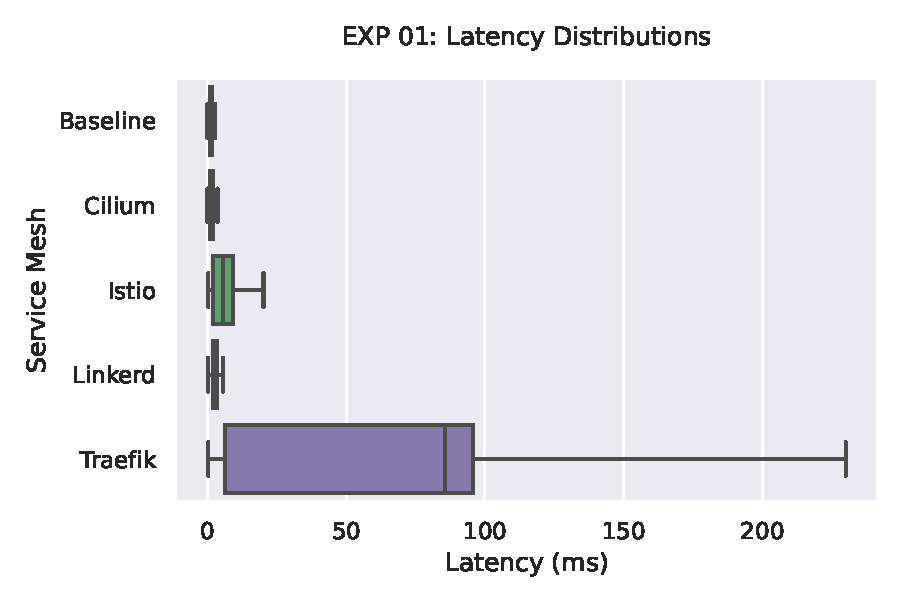
\includegraphics[width=\linewidth]{5_experimental_evaluation/figures/exp_01-latency-boxplot.pdf}

    \caption{\ref{exp:design:1} - Box plot - Latency per Service Mesh.}
    
    \label{fig:appendix:exp:result:01:latency:boxplot}
\end{figure}


\begin{figure}[h]
    \centering
    
    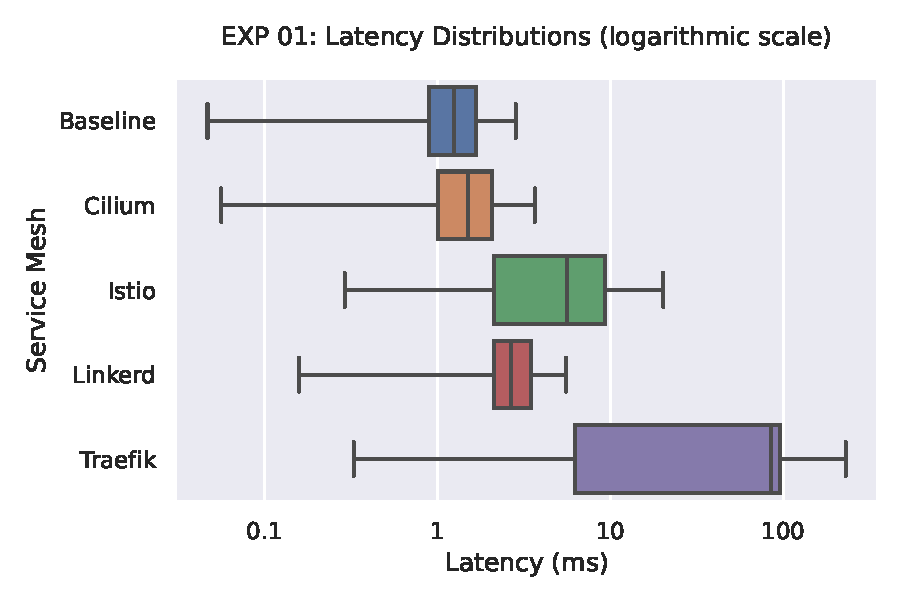
\includegraphics[width=\linewidth]{5_experimental_evaluation/figures/exp_01-latency-boxplot-log.pdf}

    \caption{\ref{exp:design:1} - Box plot - Latency per Service Mesh (logarithmic scale).}
    
    \label{fig:appendix:exp:result:01:latency:boxplot-log}
\end{figure}

\begin{figure}[h]
    \centering
    
    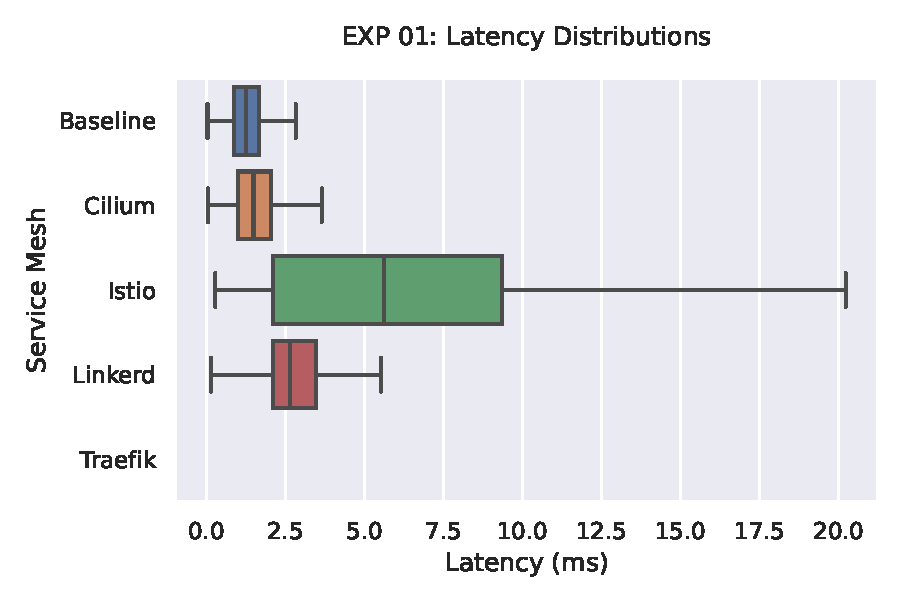
\includegraphics[width=\linewidth]{5_experimental_evaluation/figures/exp_01-latency-boxplot-no-traefik.pdf}

    \caption{\ref{exp:design:1} - Box plot - Without Traefik.}
    
    \label{fig:appendix:exp:result:01:latency:boxplot-no-traefik}
\end{figure}


\begin{figure}[h]
    \centering
    
    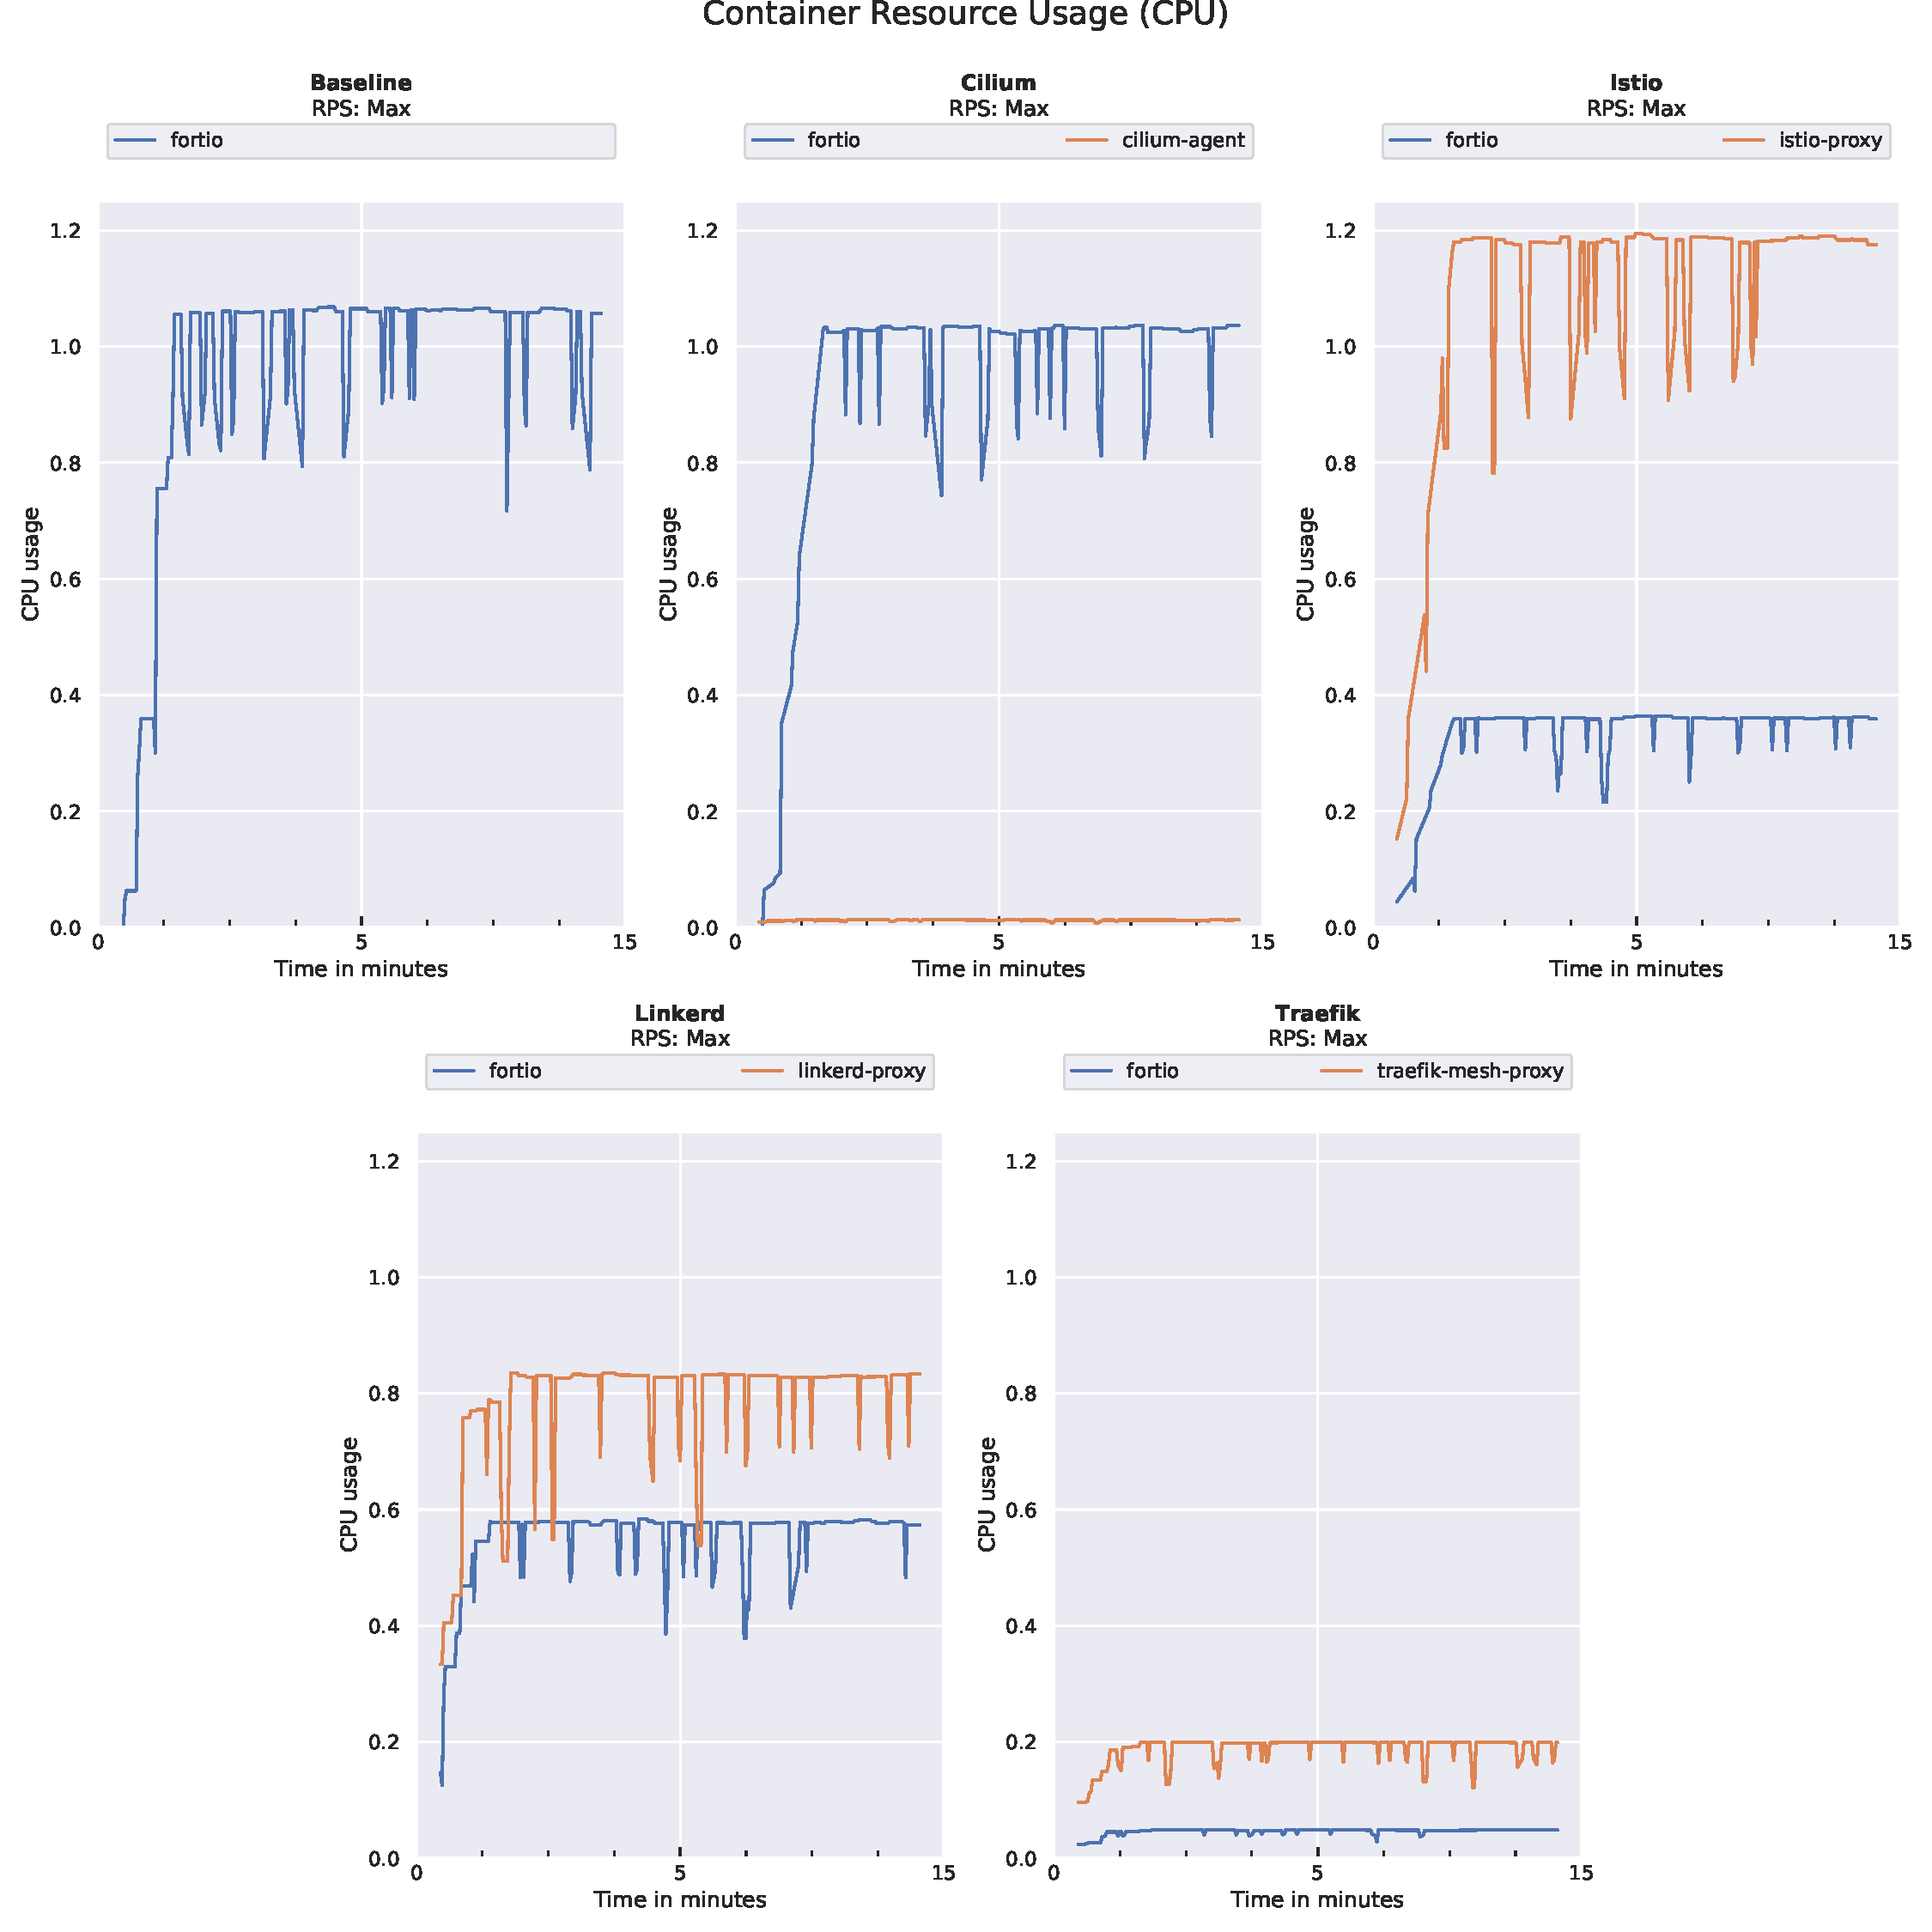
\includegraphics[width=\linewidth]{5_experimental_evaluation/figures/exp_01-cpu-results.pdf}

    \caption{\ref{exp:design:1} - CPU utilization over time.}
    
    \label{fig:appendix:exp:result:01:cpu:timeline}
\end{figure}


\begin{figure}[h]
    \centering
    
    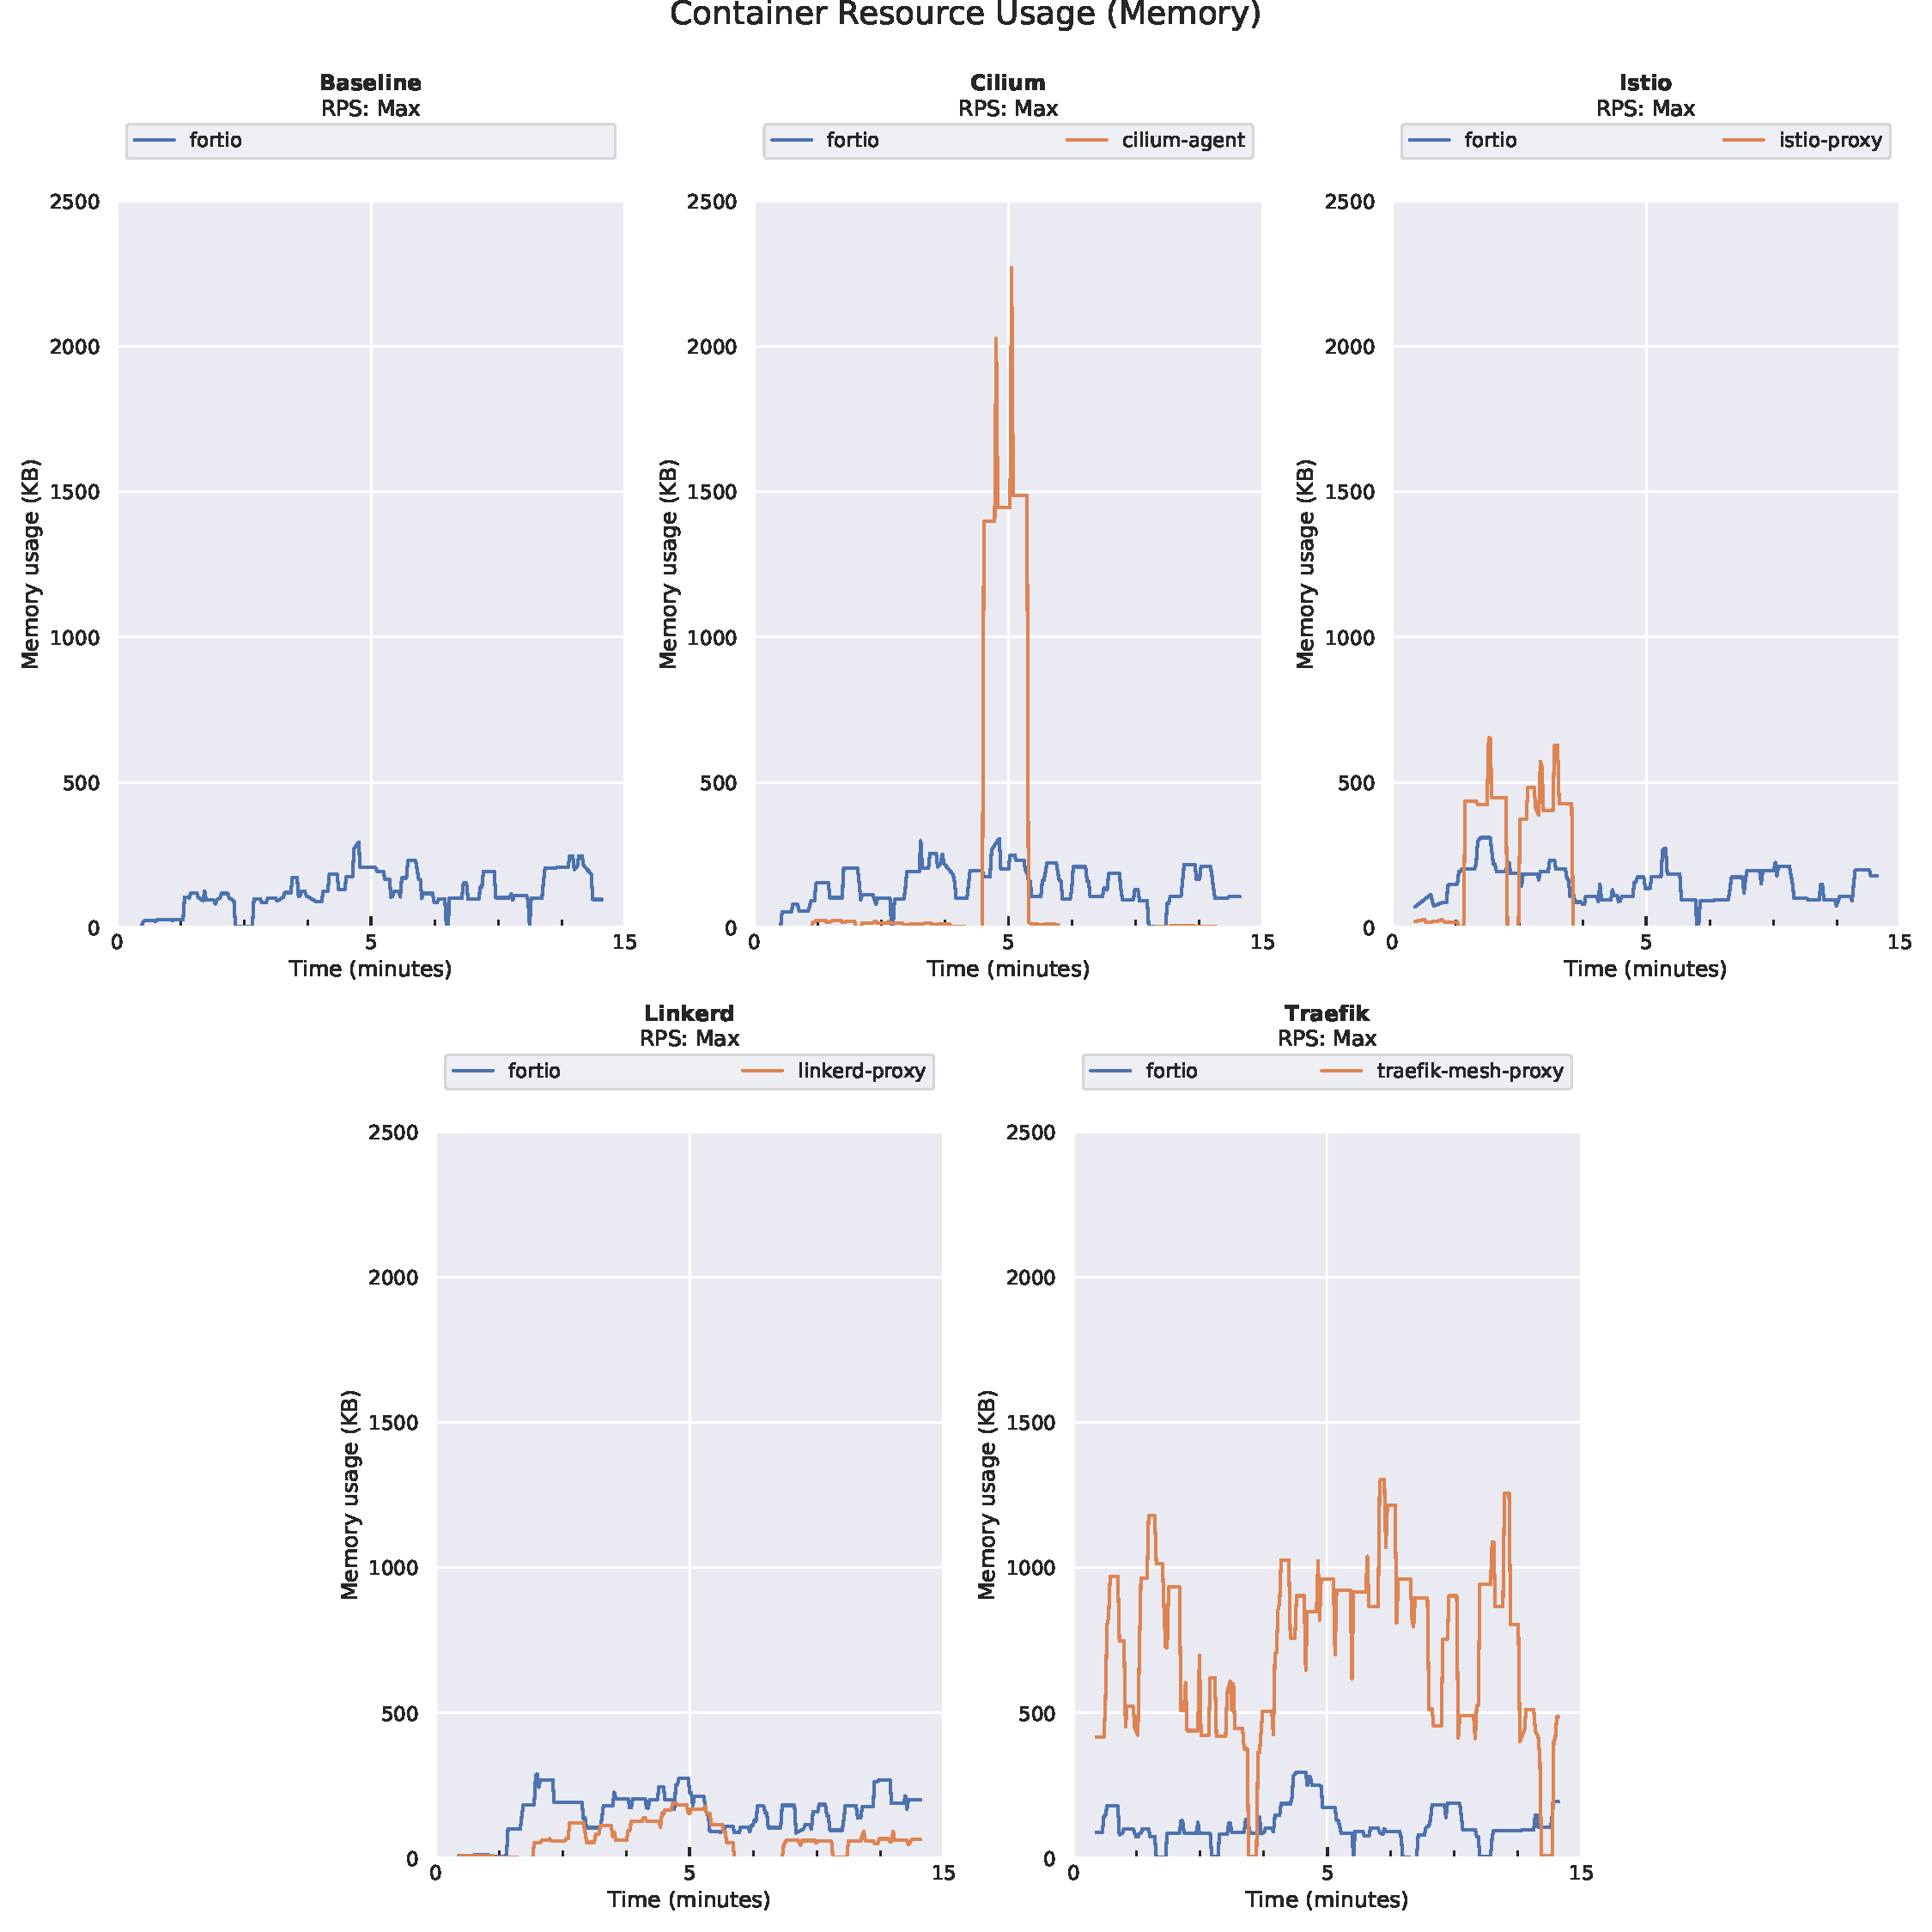
\includegraphics[width=\linewidth]{5_experimental_evaluation/figures/exp_01-memory-results.pdf}

    \caption{\ref{exp:design:1} - Memory consumption over time.}
    
    \label{fig:appendix:exp:result:01:memory:timeline}
\end{figure}


\begin{figure}[h]
    \centering
    
    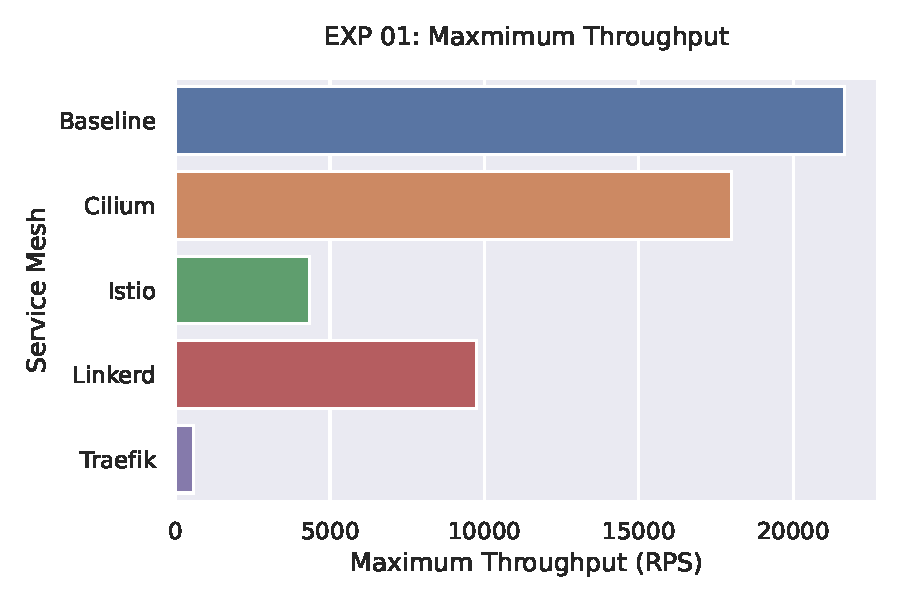
\includegraphics[width=\linewidth]{5_experimental_evaluation/figures/exp_01-throughput-barchart.pdf}

    \caption{\ref{exp:design:1} - Bar Chart - Maximum Throughput per mesh.}
    
    \label{fig:appendix:exp:result:01:throughput:barchart}
\end{figure}


\section{Experiment 2 Results}

\begin{figure}[h]
    \centering
    
    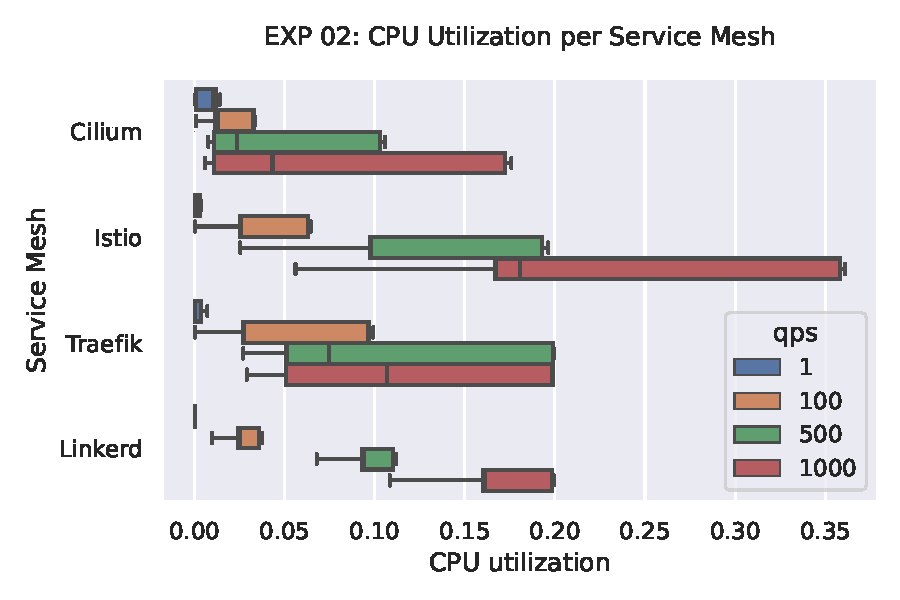
\includegraphics[width=\linewidth]{5_experimental_evaluation/figures/exp_02-cpu-boxplot.pdf}

    \caption{\ref{exp:design:2} - Box Plot - CPU utilization.}
    
    \label{fig:appendix:exp:result:02:cpu-boxplot}
\end{figure}


\section{Experiment 3 Results}

\section{Experiment 4 Results}
